\begin{frame}[allowframebreaks]{Motivation}
	\textbf{\textcolor{blue}{Why Secret Sharing?}}
	\begin{itemize}
		\item Allows splitting a secret into \emph{shares} so that only certain subsets of participants $\Gamma$ can reconstruct the secret information.
		\item Avoid single points of failure: Attribute-Based Encryption (\textbf{ABE}) - key management, authority, or storage.
		\item Foundational block for many cryptographic protocols: secure multi-party computation, threshold criptography, access control, multi-factor authentication.
	\end{itemize}
	
	\begin{figure}
		\centering
		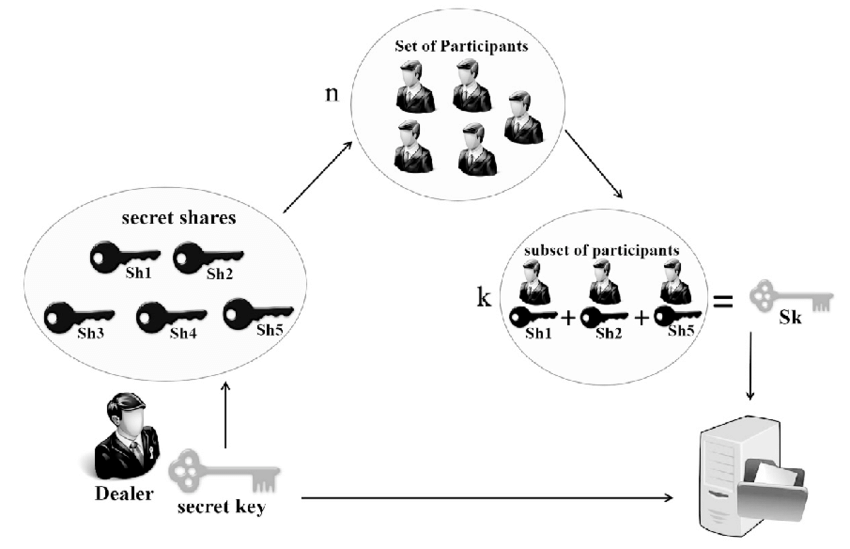
\includegraphics[scale=0.3]{fig/fig-threshold-secret-sharing.png}
		\caption{The notion of Threshold Secret Sharing \cite{gutub2020}}
	\end{figure}
\end{frame}

\begin{frame}{Access Structures}
	\begin{itemize}
		\item Parties: \(\mathcal{P} = \{P_1,\dots,P_n\}\).
		\item Access structure \(\mathcal{A}\subseteq 2^{\mathcal{P}}\): sets that can reconstruct.
		\item \textbf{Monotone} requirement: if \(A\in\mathcal{A}\) and \(A\subseteq B\), then \(B\in\mathcal{A}\).
	\end{itemize}
\end{frame}

\begin{frame}{Perfect Secret Sharing - \cite{beimel2011secret}}
	Let secret \(S\) be random and shares be random variables \(\{S_i\}\). The domain of secrets \(S\) (given by its shares) is a secret sharing scheme realizing an access structure \(\mathcal{A}\) if:
	\begin{itemize}
		\item \textbf{Correctness:} For every \(A\in\mathcal{A}\), \(S\) is determined by \(\{S_i : P_i\in A\}\).
		\item \textbf{Perfect privacy:} For every \(T\notin\mathcal{A}\), shares reveal no information:
		\[
			I(S;\{S_i: P_i\in T\}) = 0
			\quad\Longleftrightarrow\quad
			H(S\mid \{S_i: i\in T\}) = H(S).
		\]
		\item Lower bound intuition: in any perfect scheme, each non-redundant party’s share must be at least as large as the secret.
	\end{itemize}
\end{frame}